\chapter{Results}
\label{ch:results}


\section{Evolution of Patterns}
\label{sec:pattern evolution}

This Section gives an overview how the EOF patterns change over the time, also comparing the differences of the two chosen climate scenarios, which represent the extremes of climate change handling.   

\subsection{Evolution of Encoded Variability}



\begin{figure}[htb]
  \begin{center}
    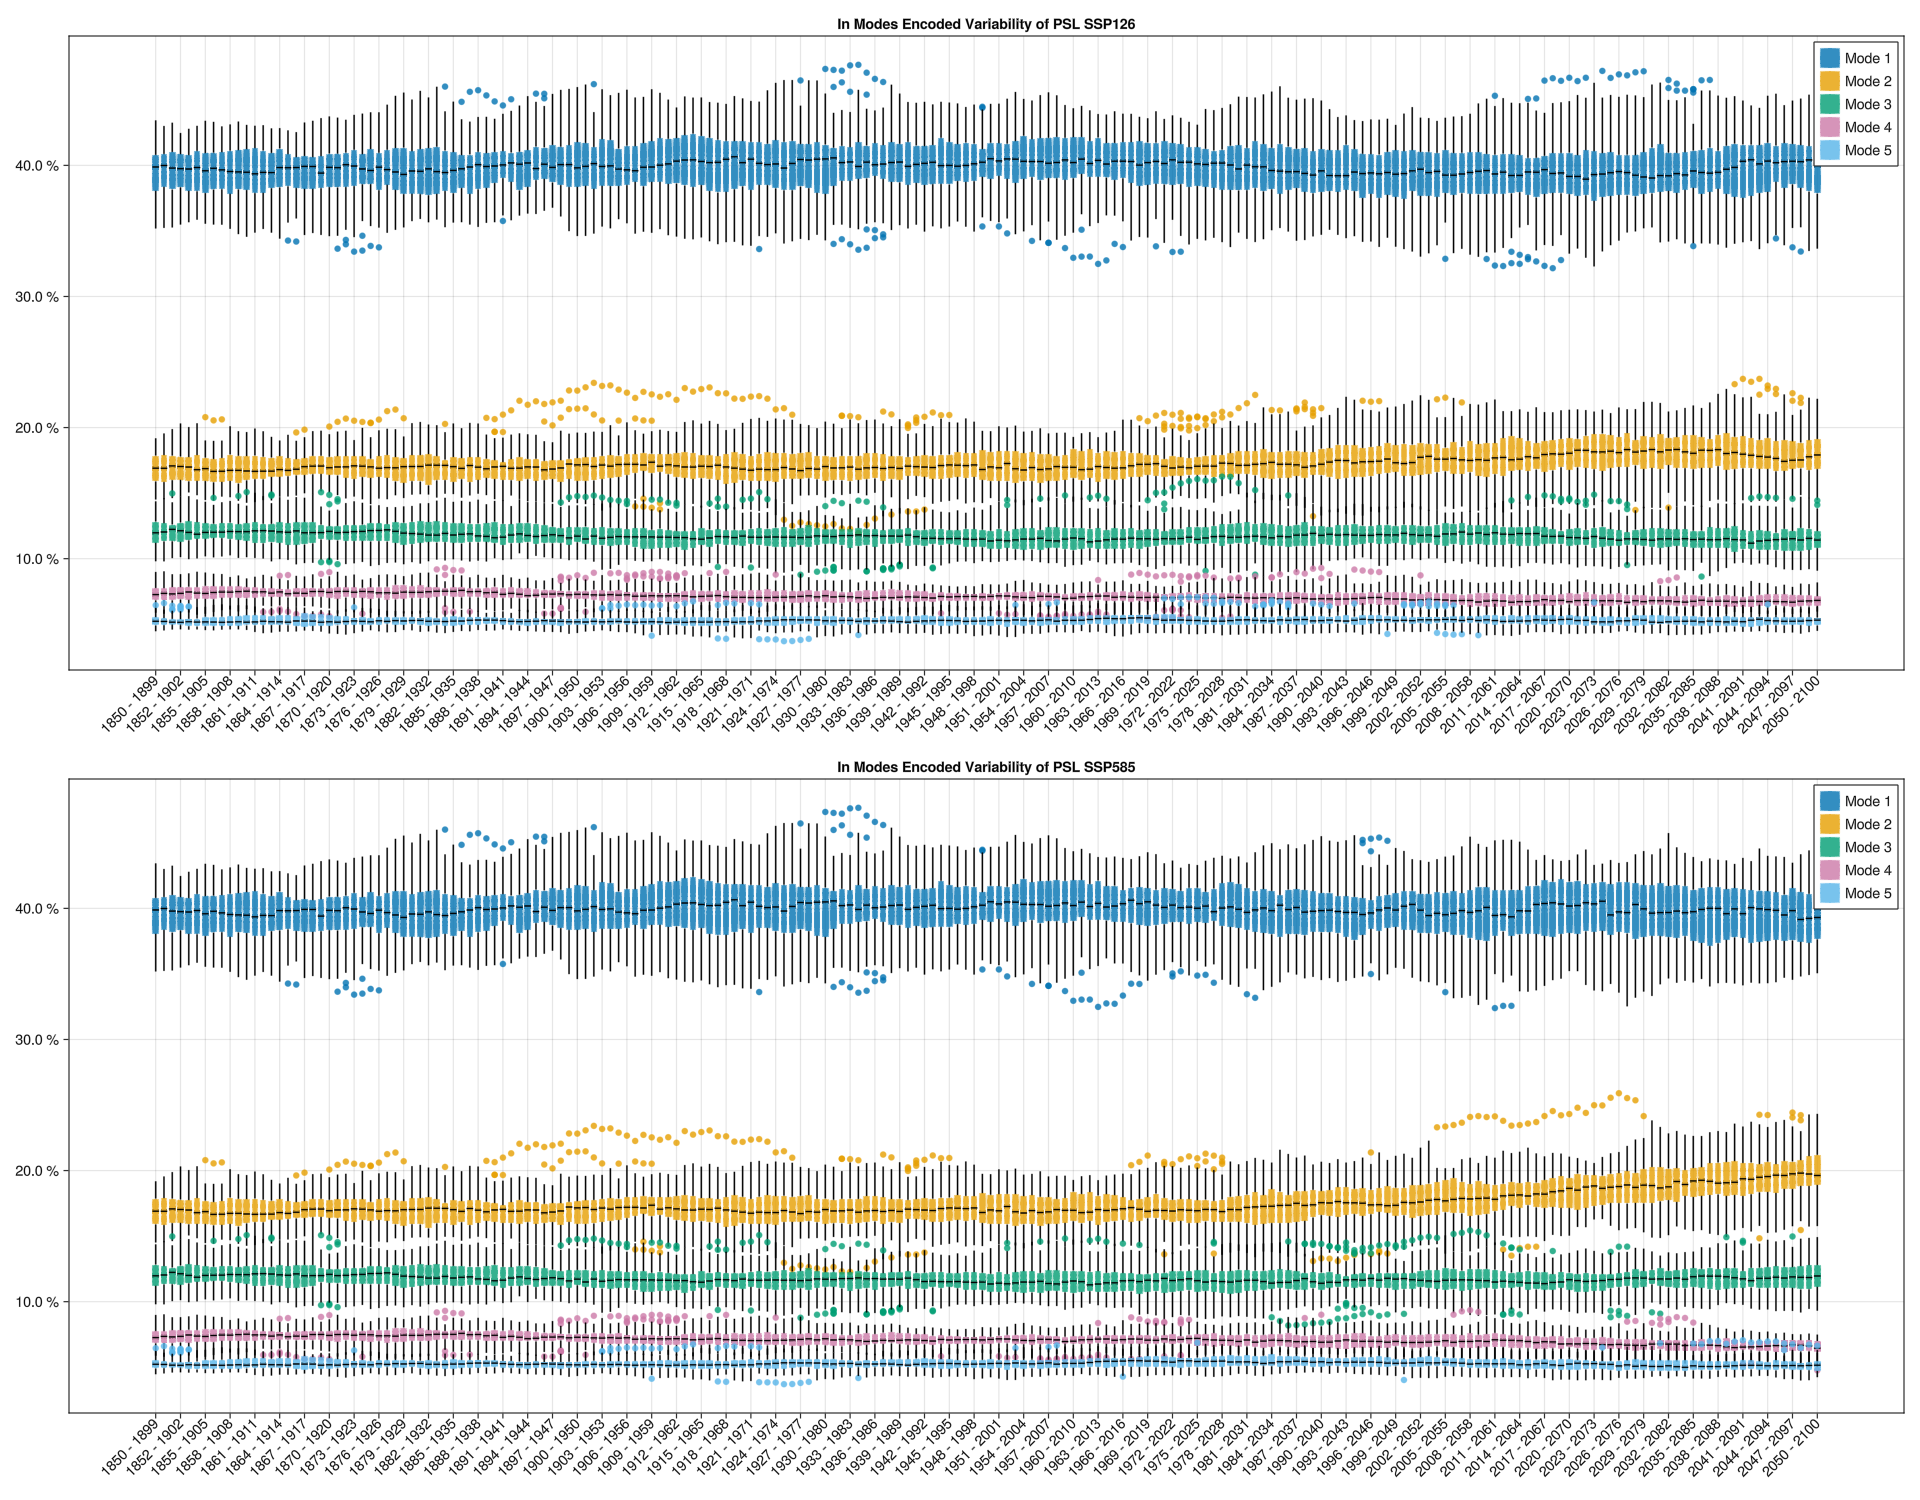
\includegraphics[width=0.85\textwidth]{figures/mode_variability_psl_50seasons.png}
  \end{center}
  \caption{Boxplot of the variability encoded in the top five modes of PSL EOF.}\label{fig:psl mode variability}
\end{figure}

The first simple evaluation is to look at the change of share of variability encoded by each EOF (see Equation~\ref{eq:eof variance calculation}). 
The results are displayed in boxplots, with the colored bar being $50\%$  of the members. 
The whiskers are 1.5 the size of the interquartile range (distance between upper and lower and of the colored bar), any data point outside that is considered an outlier and represented with dots. 


Figure~\ref{fig:psl mode variability} shows that there is no significant change in the SSP126 scenario in any way. 
The five most significant modes stay pretty much the same across the studied 250-year time period, with the primary mode (NAO) encoding around $39\%$ (median) of the whole dataset variability in each time scope, with fluctuations of the interquartile range ($50\%$ of the data) introduced by the members of the simulations being around $\pm 2\%$, with no significant trend over the years. 
The secondary mode (EAP) median stays around $17\%$, with the quartiles being $\pm 1\%$. 
The median variability encoded by EOFs 3,4 and 5 is around $13\%$, $8\%$, and $5\%$, respectively. 
Comparing it to the SSP585 scenario, it is obvious that there is very little to no change in Modes 3-5 and 1. 
But interestingly, the median variability encoded by the secondary mode rises from the $17\%$ in the 1850 - 1900 scope to around $20\%$ in the last one, exposing a clear trend over the course of climate change.   


\begin{figure}[hbt]
  \begin{center}
    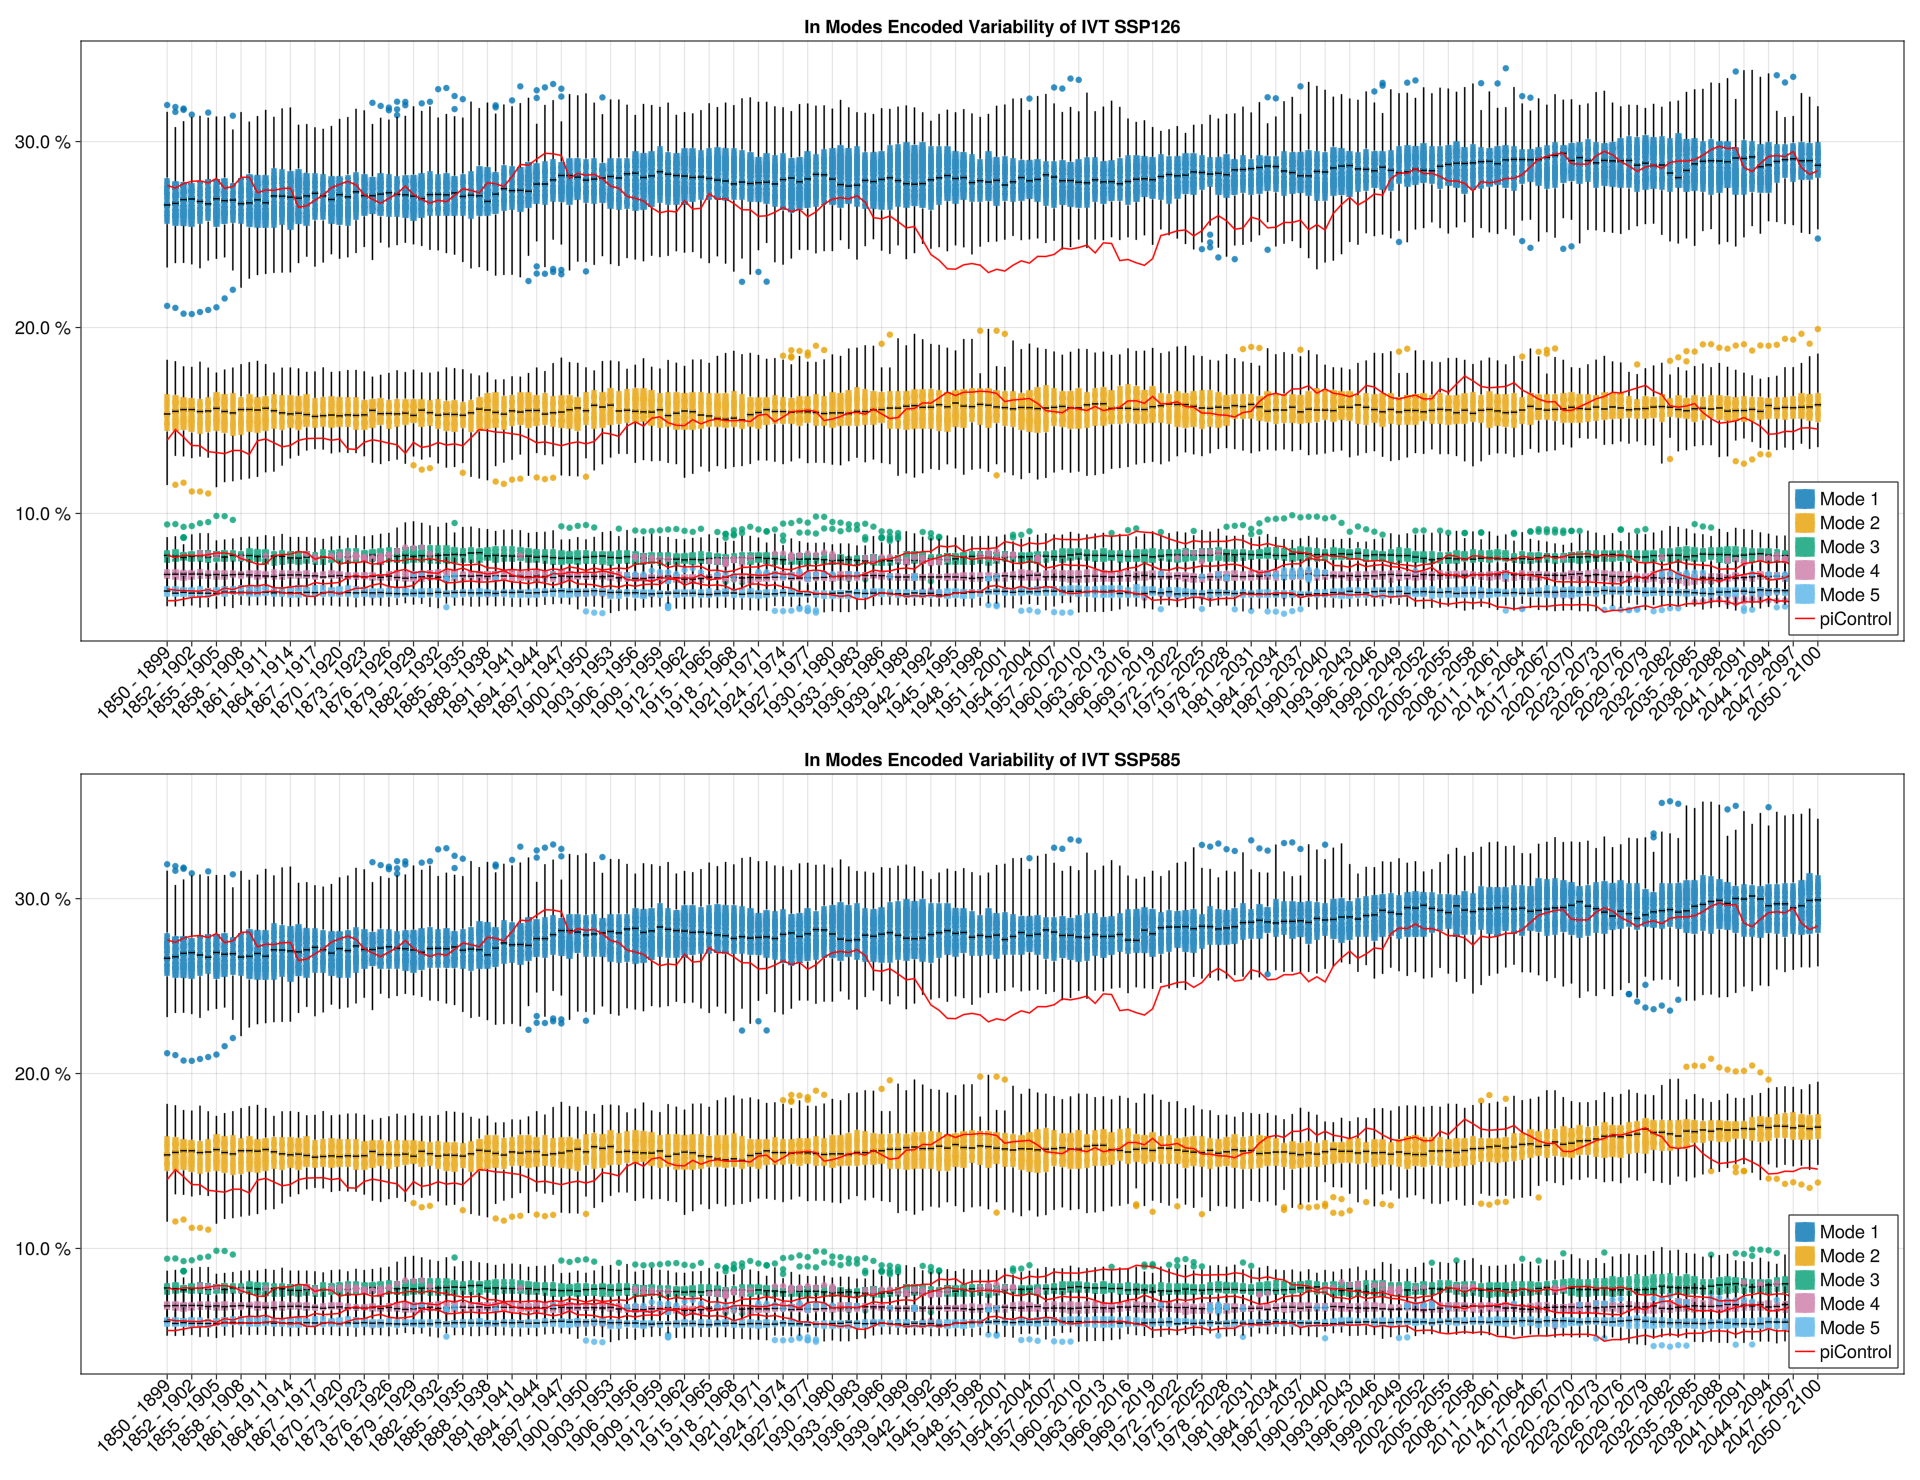
\includegraphics[width=0.85\textwidth]{figures/mode_variability_ivt_50seasons.png}
  \end{center}
  \caption{Same as Figure~\ref{fig:psl mode variability} but with IVT}\label{fig:ivt mode variability}
\end{figure}

The same analysis with the IVT patterns (Figure~\ref{fig:ivt mode variability}) reveal a general upwards trend in the primary mode of IVT, from median $26\%$ in the first window to around $28\%$ in the last. 
This trend is very similar in both SSP126 and SSP 585. 
Modes 3,4 and 5 also look very similar in both evaluated scenarios, with a median encoded variability of $8\%$, $6\%$, and $5\%$. 
Similar to Figure~\ref{fig:psl mode variability}, the secondary mode (representing around $15\%$ of variability) shows upward trend in scenario SSP585 to around $17\%$, which is not recognizable in the SSP126 scenario. 

\begin{figure}[htb]
  \begin{center}
    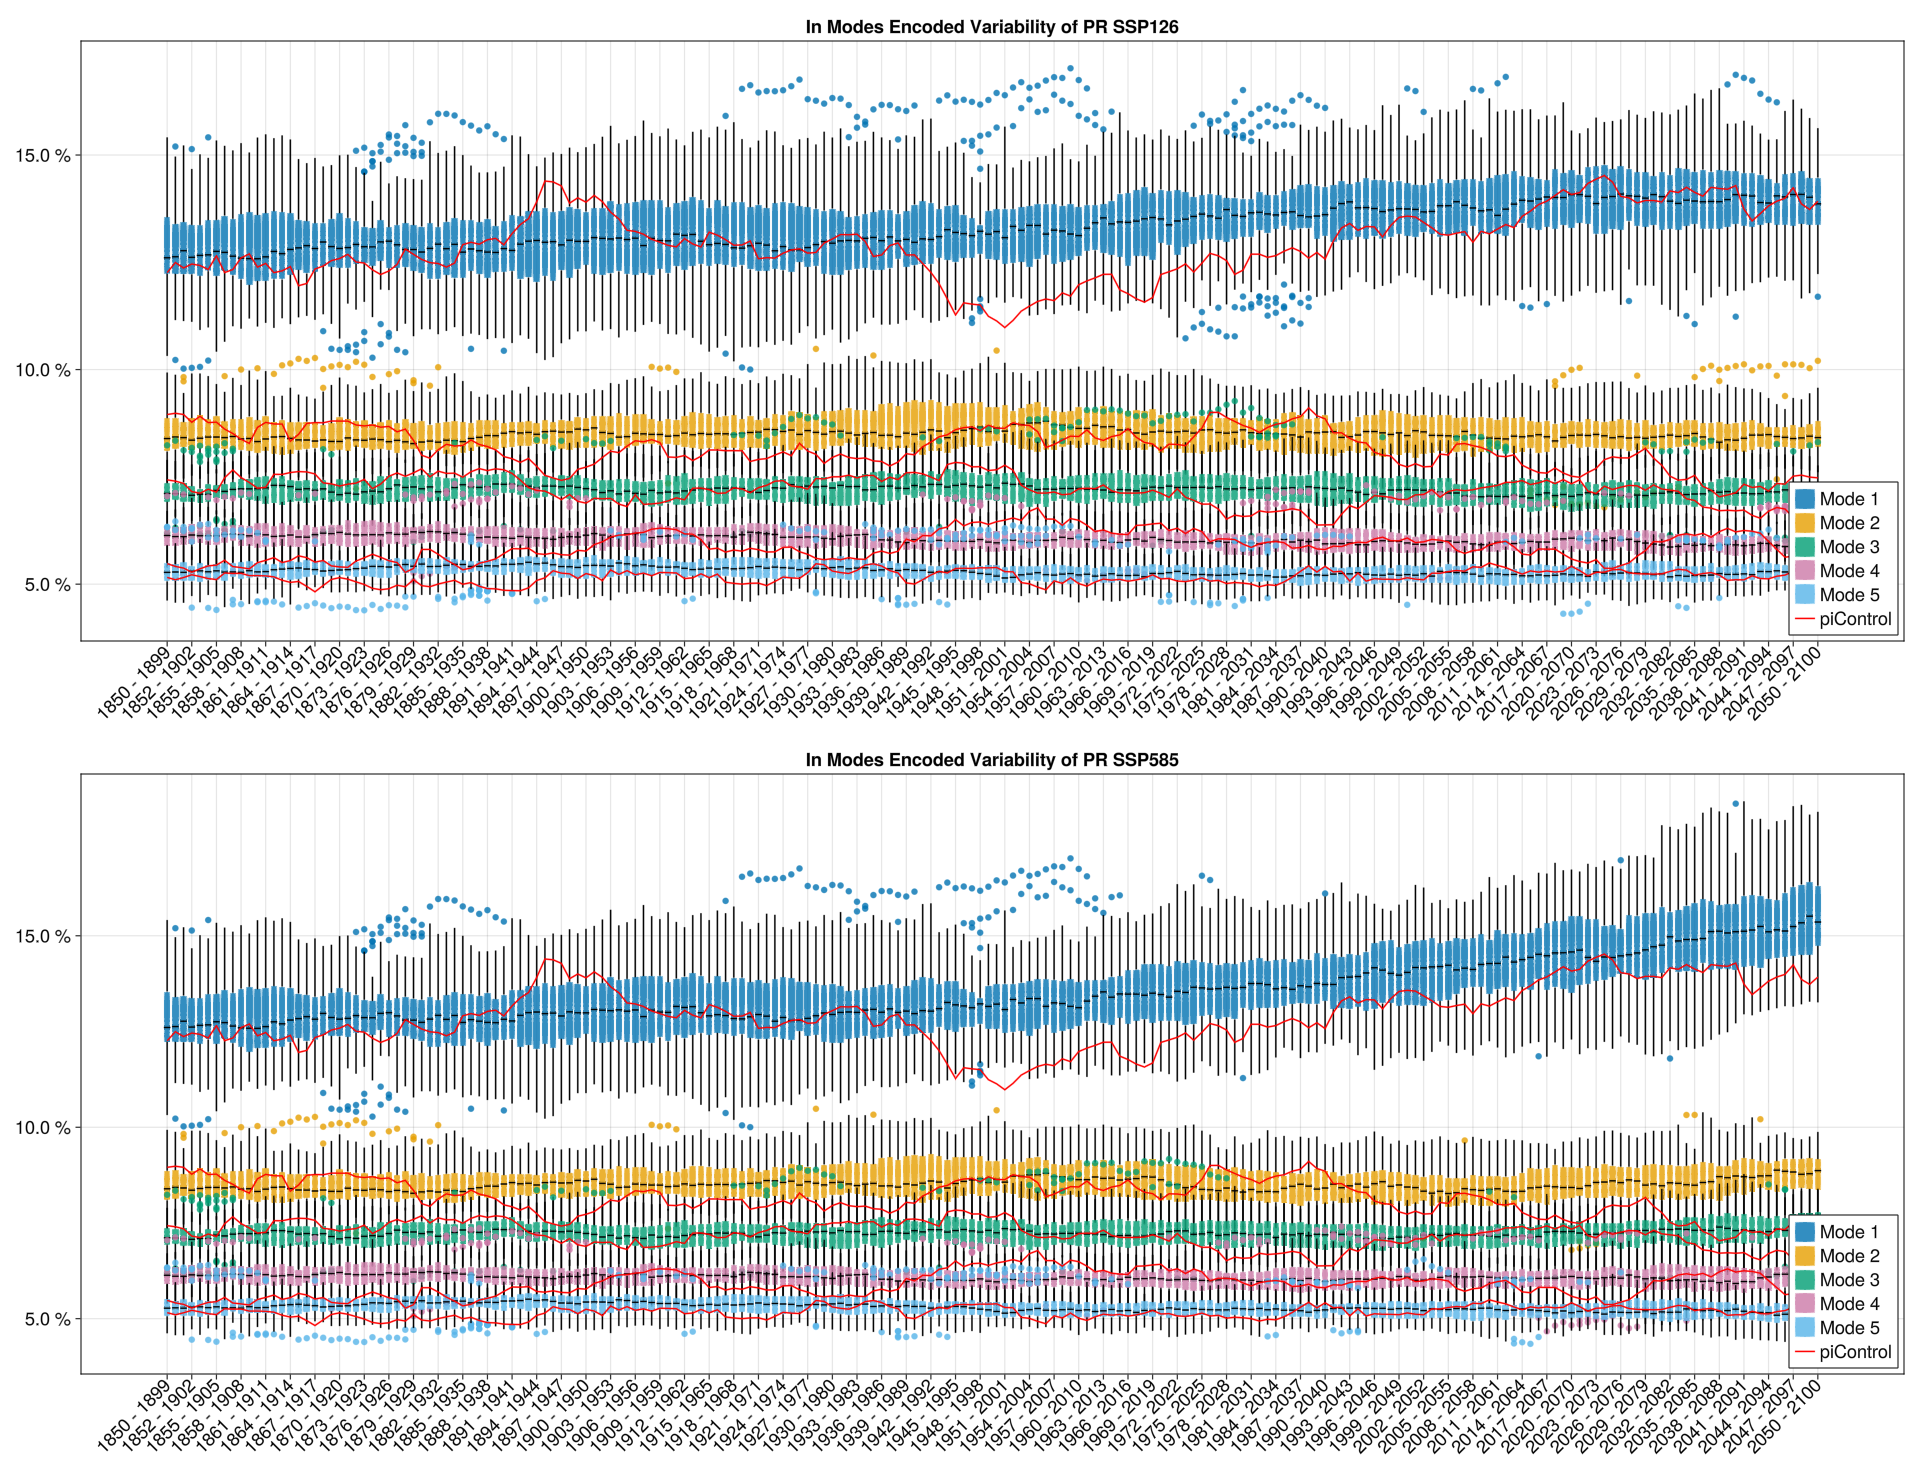
\includegraphics[width=0.85\textwidth]{figures/mode_variability_pr_50seasons.png}
  \end{center}
  \caption{Same as Figure~\ref{fig:psl mode variability} but with precipitation}\label{fig:pr mode variability}
\end{figure}

The comparison of mode variability evolution of precipitation EOFs (Figure~\ref{fig:pr mode variability}) shows no significant changes of modes 3,4, and 5 between both evaluated scenarios. 
Those encode on median $5\%$, $6\%$ and $6.5\%$ with small fluctuations introduced by the members. 
Mode 2 also looks very similar in both scenarios, with a median encoded variability of around $8.5\%$. 
The primary EOF on the other shows significant differences across scenarios: While it has a far greater variability across members then the other modes and follows a general upwards trend in both SSP126 and SSP585, it is more pronounced in the latter. 
It evolves from around $12.5\%$ in the 1850-1900 window to around $14\%$ in SSP126 and $15.5\%$ in SSP585.  


\subsection{Evolution of Spatial Patterns}

\begin{figure}
  \begin{center}
    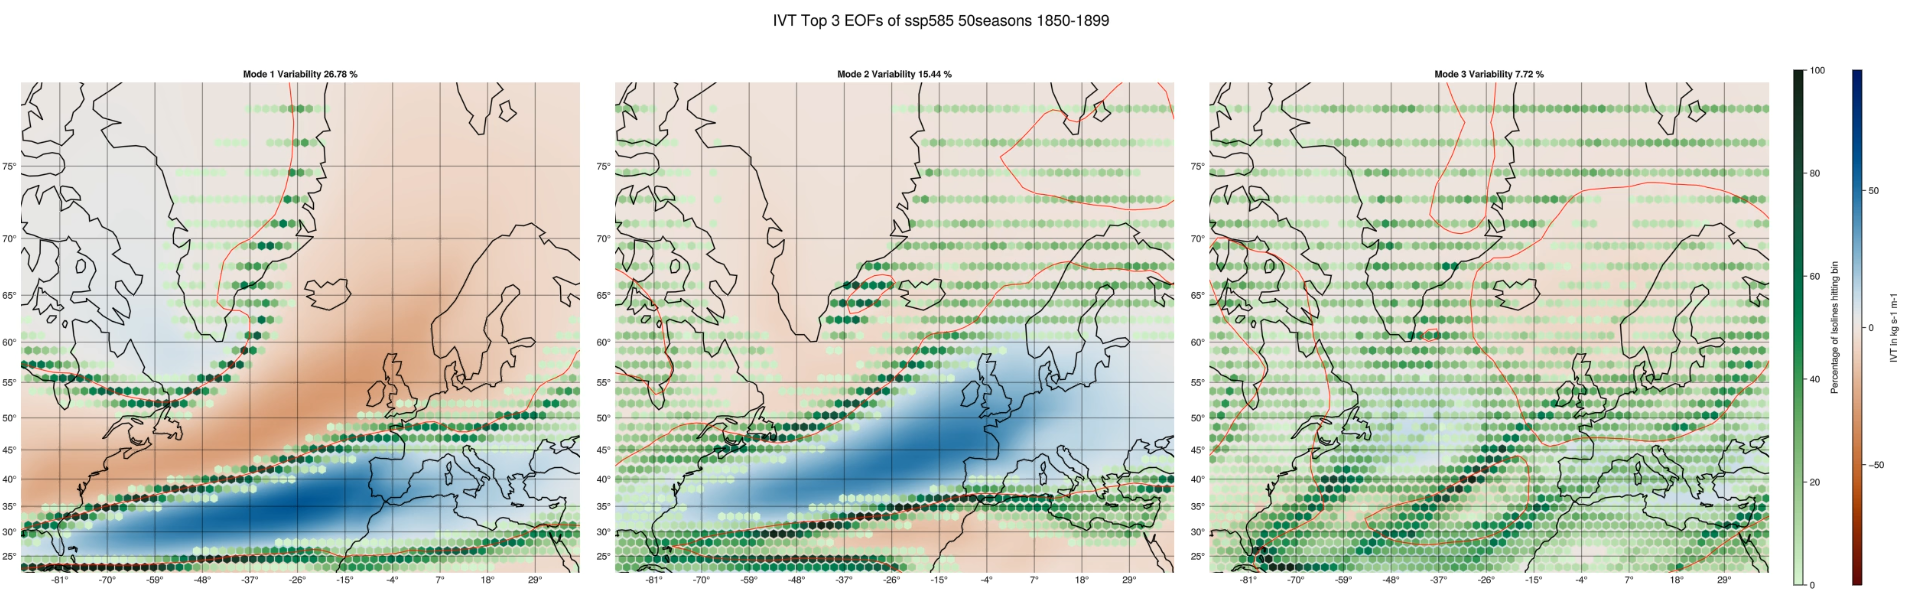
\includegraphics[width=0.95\textwidth]{figures/ivt_spat_patterns_hexbin_18501899_ssp585_50seasons.png}
    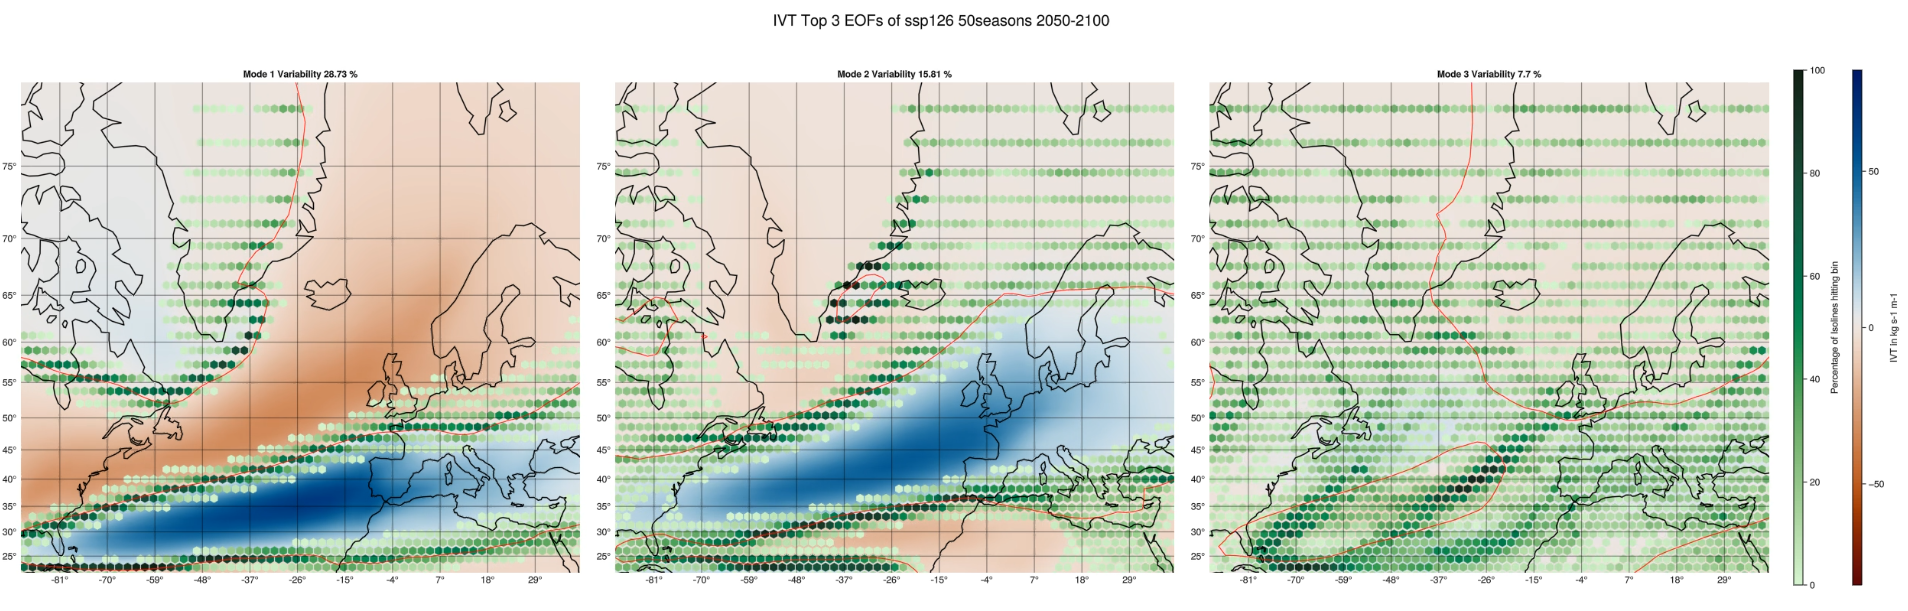
\includegraphics[width=0.95\textwidth]{figures/ivt_spat_patterns_hexbin_20502100_ssp126_50seasons.png}
    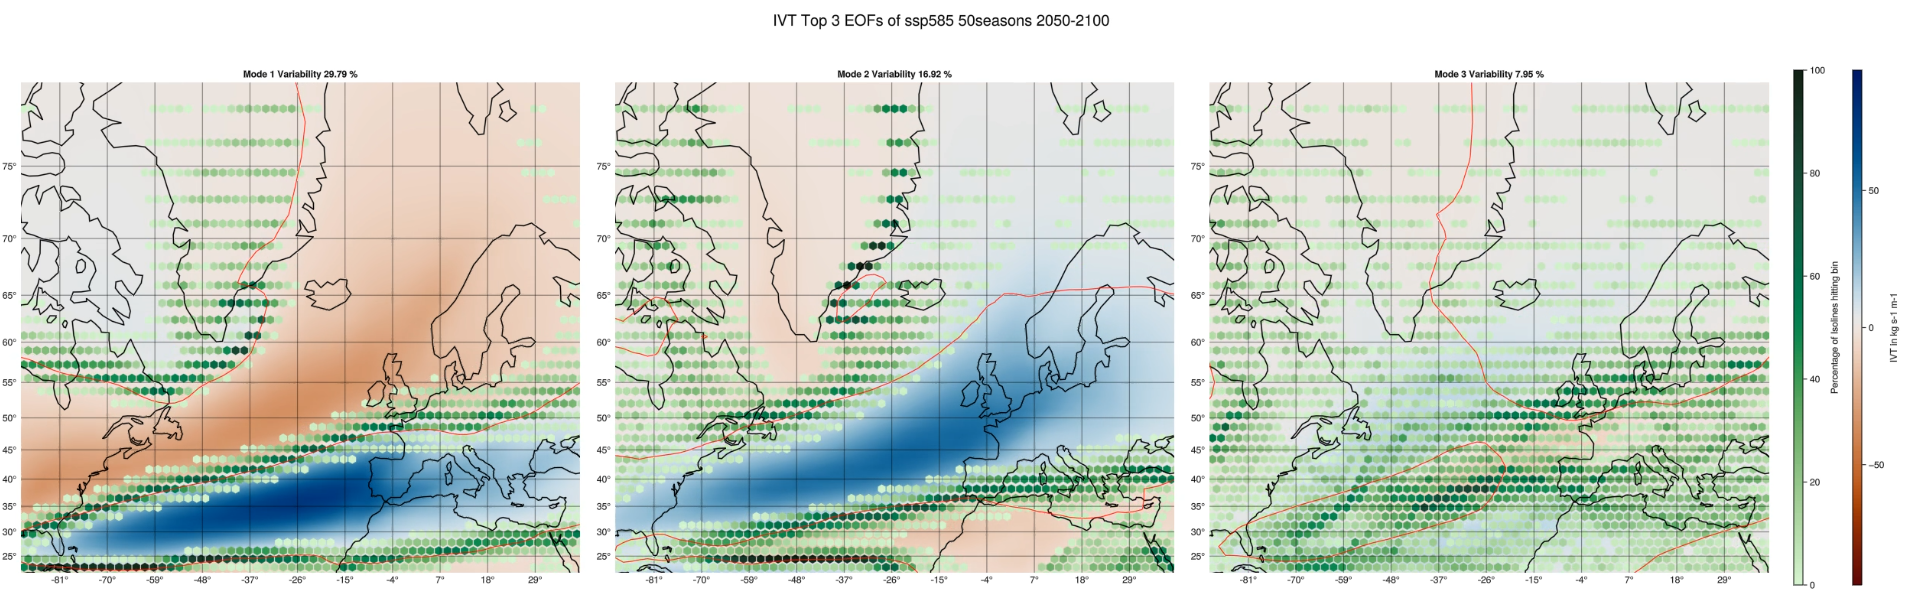
\includegraphics[width=0.95\textwidth]{figures/ivt_spat_patterns_hexbin_20502100_ssp585_50seasons.png}
  \end{center}
  \caption{The top three EOFs of IVT data, with a 50 winter scope and hexbins visualizing the variability introduced by simulation members. The top row displays the state in the historical simulation (second half of 19th century), while middle (SSP126) and bottom (SSP585) display the state in the second half of the 21st century. The red line shows the contour line of zero of the preindustrial control simulation. }\label{fig:ivt eof evolution}
\end{figure}



\begin{figure}
  \begin{center}
    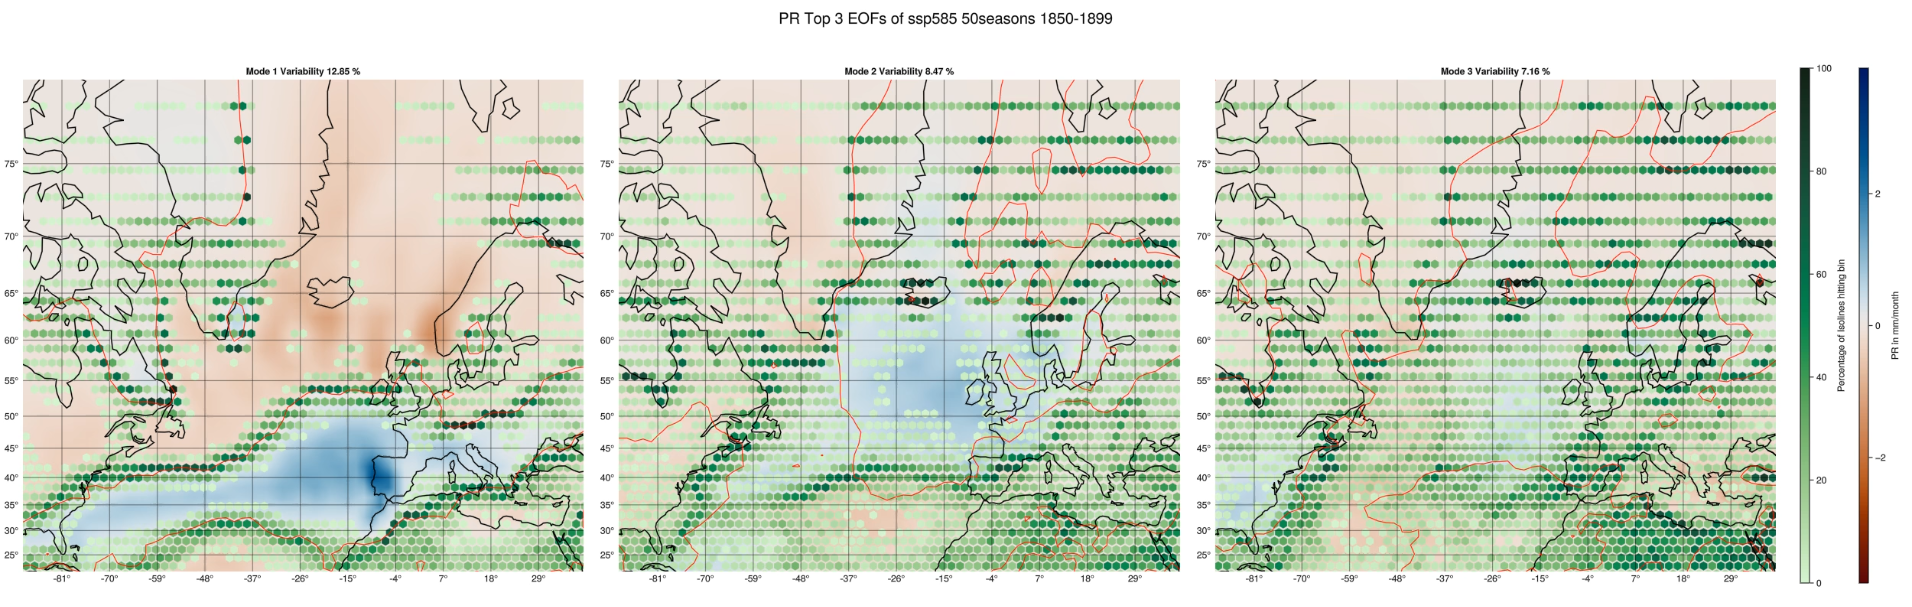
\includegraphics[width=0.95\textwidth]{figures/pr_spat_patterns_hexbin_18501899_ssp585_50seasons.png}
    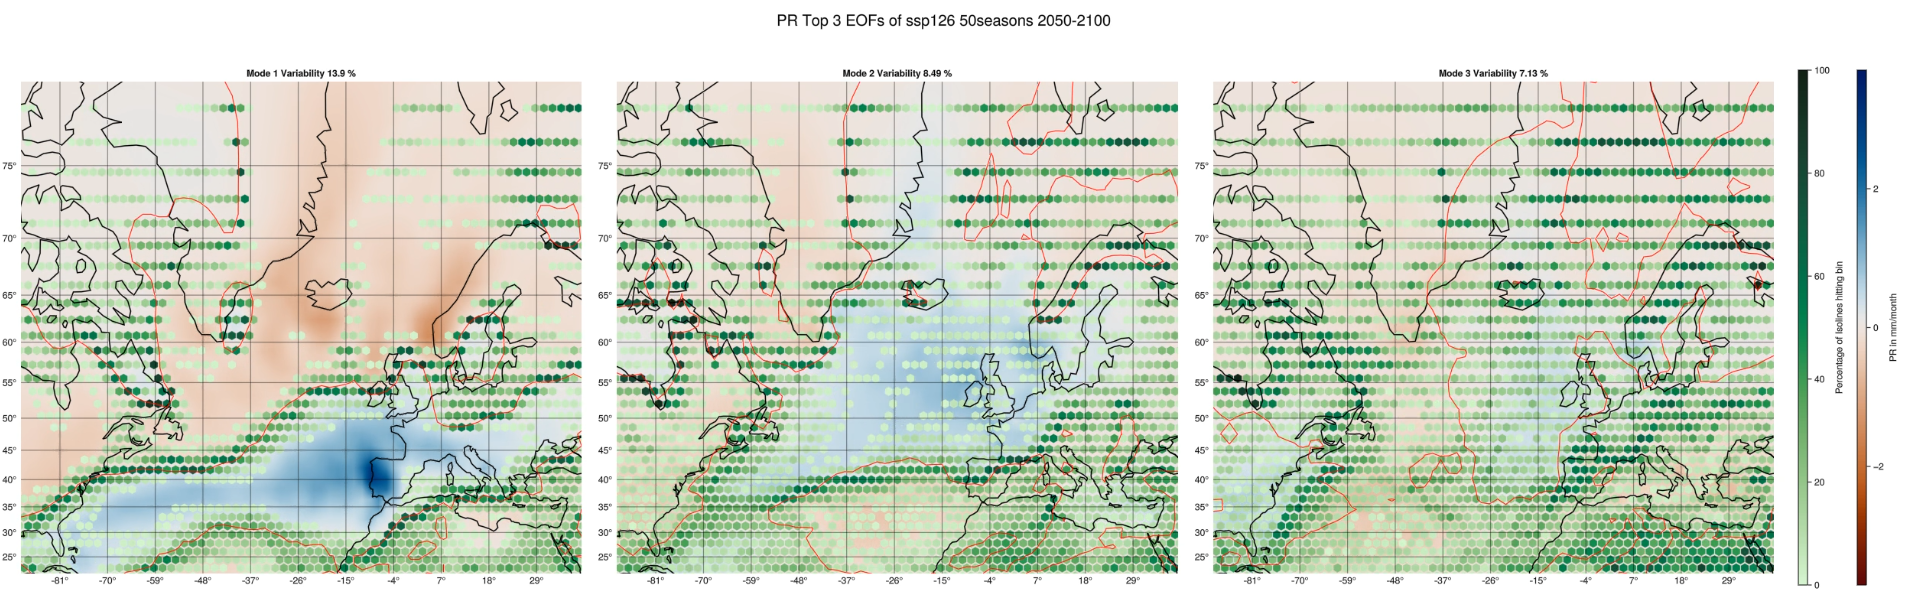
\includegraphics[width=0.95\textwidth]{figures/pr_spat_patterns_hexbin_20502100_ssp126_50seasons.png}
    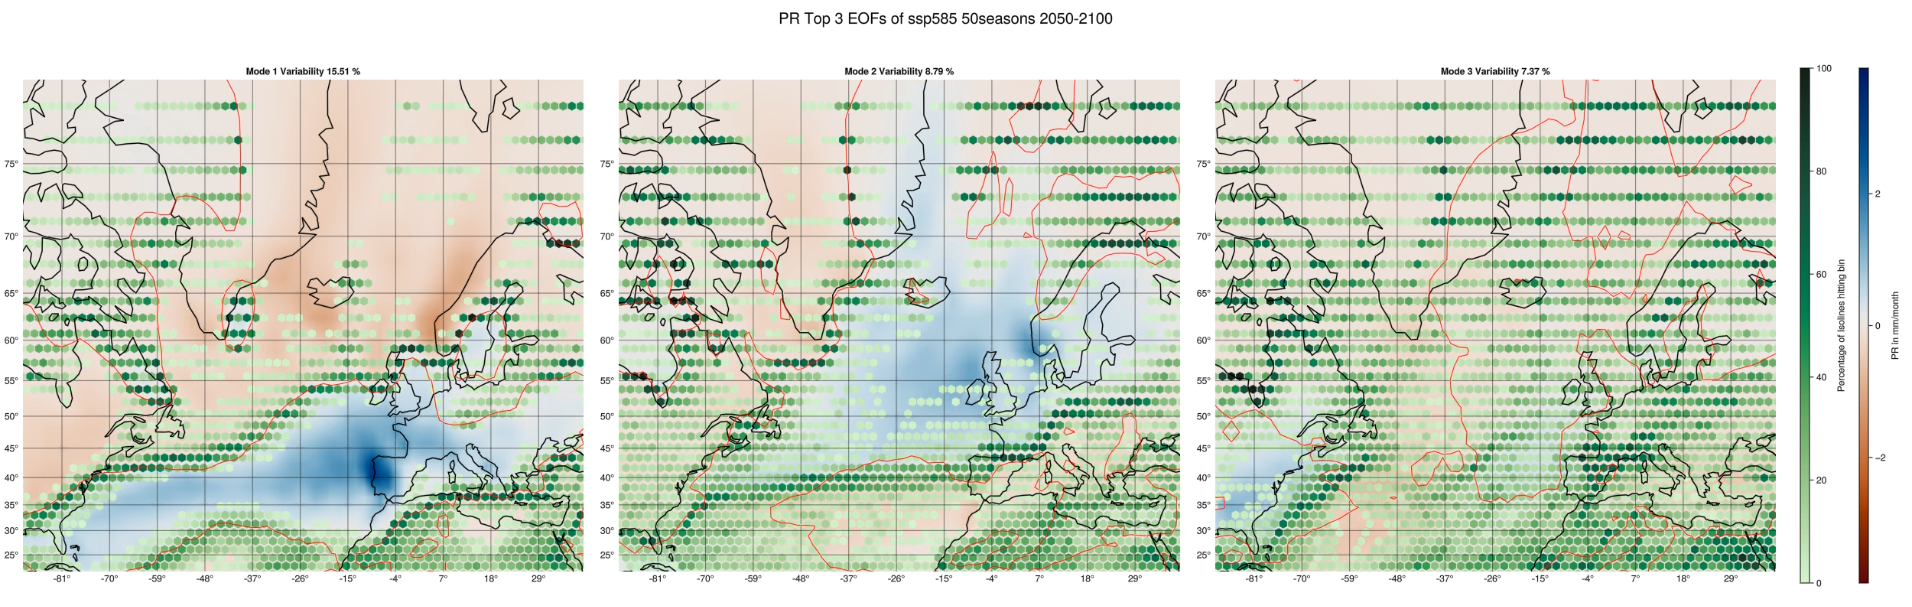
\includegraphics[width=0.95\textwidth]{figures/pr_spat_patterns_hexbin_20502100_ssp585_50seasons.png}
  \end{center}
  \caption{Same as Figure~\ref{fig:ivt eof evolution}, but with precipitation data.}\label{fig:pr eof evolution}
\end{figure}

\begin{figure}
  \begin{center}
    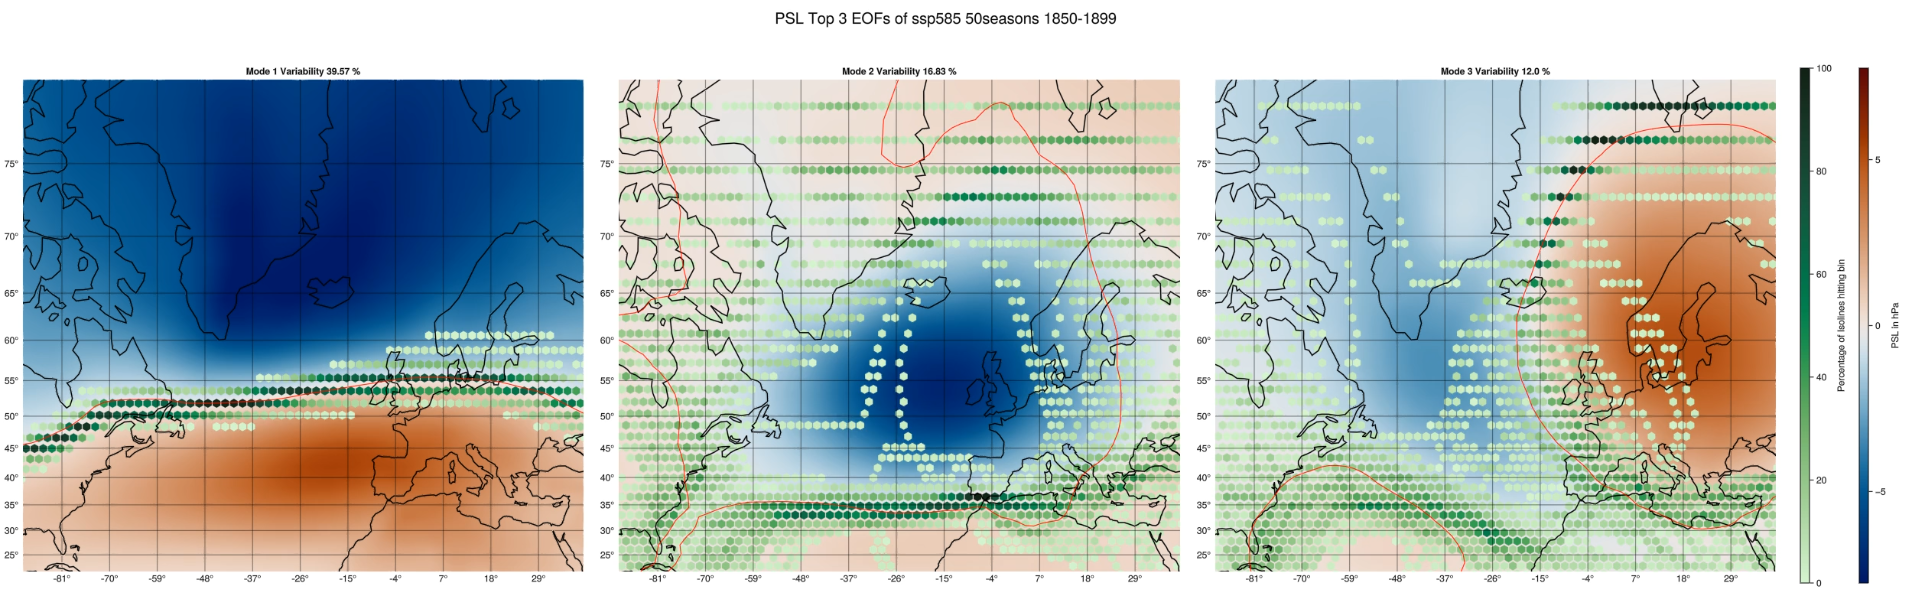
\includegraphics[width=0.95\textwidth]{figures/psl_spat_patterns_hexbin_18501899_ssp585_50seasons.png}
    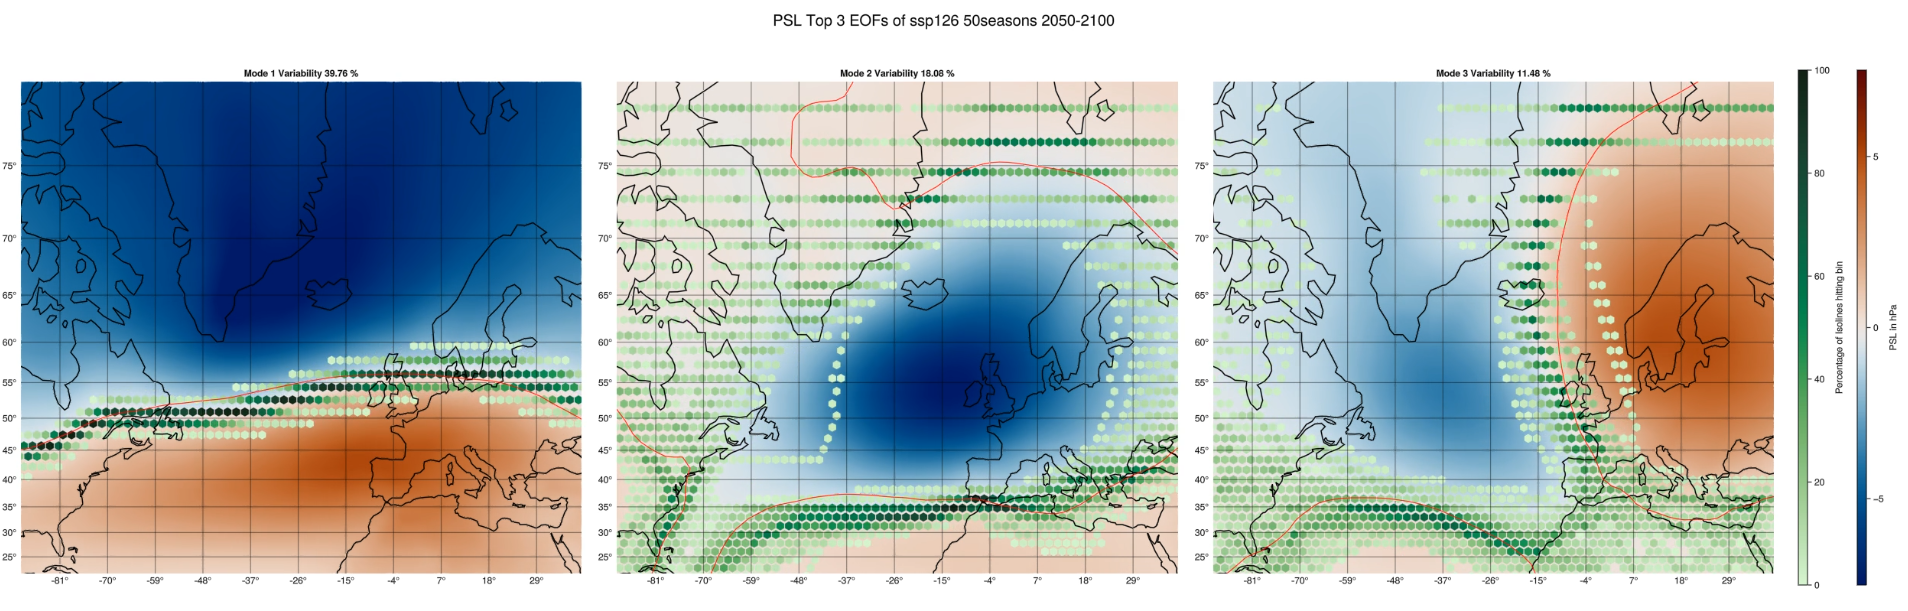
\includegraphics[width=0.95\textwidth]{figures/psl_spat_patterns_hexbin_20502100_ssp126_50seasons.png}
    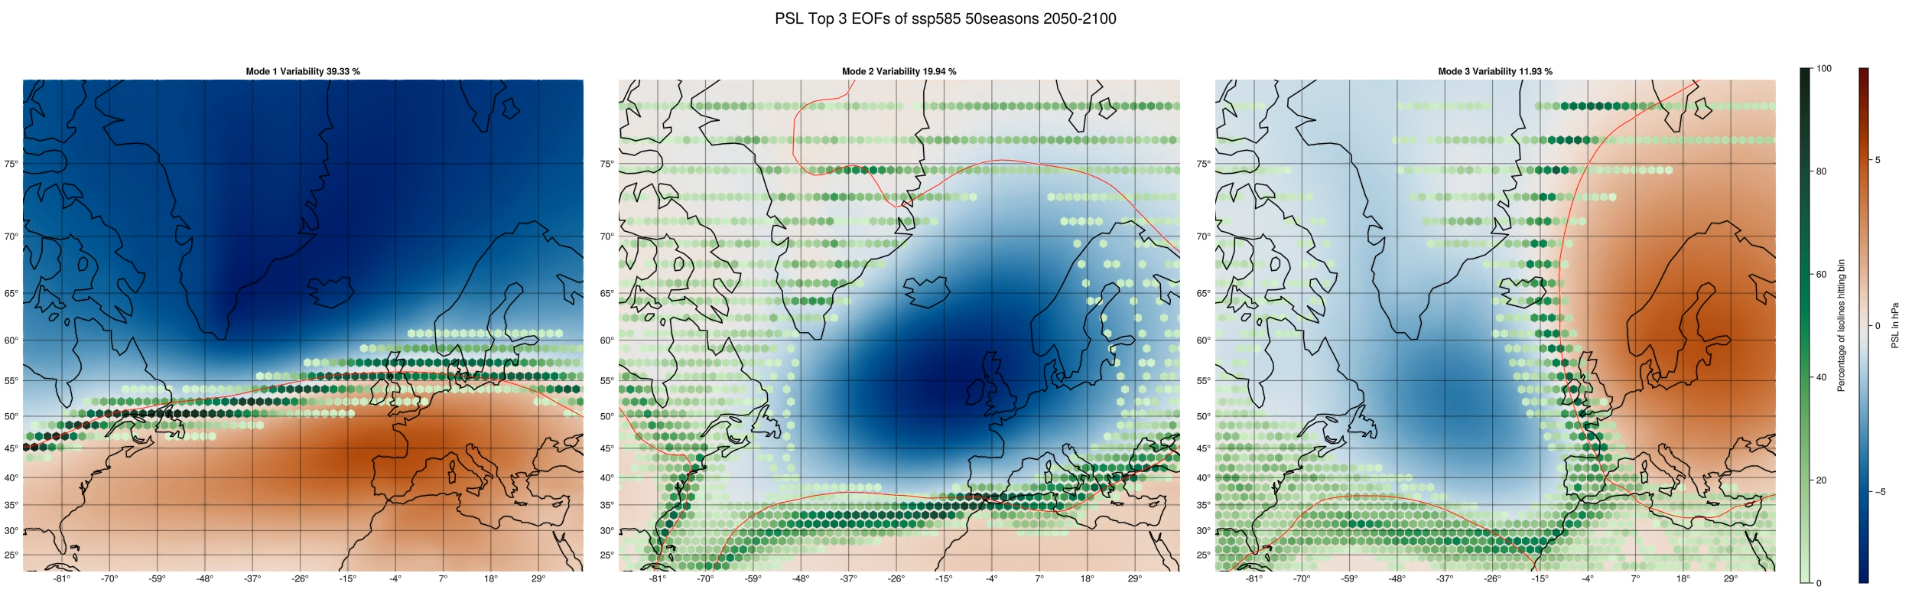
\includegraphics[width=0.95\textwidth]{figures/psl_spat_patterns_hexbin_20502100_ssp585_50seasons.png}
  \end{center}
  \caption{Same as Figure~\ref{fig:ivt eof evolution}, but with sea level pressure data.}\label{fig:psl eof evolution}
\end{figure}

\section{Relationships with other Variables}

\subsection{Relationships of EOFs}


\subsection{Relationships of EOFs with Variables}


\section{Discussion of Interpretation}
\label{sec:discussion}
